  \chapter{Нейросетевые методы машинного обучения для задач обработки естественного языка}\label{ch:ch1} 
  

\section{Определение нейросетевых методов машинного обучения}
Нейросетевые методы машинного обучения - это методы, основанные на использовании нейронных сетей. Нейронная сеть представляет собой совокупность слоев с функциями активации, таких, что подаваемые на вход данные проходят через различные слои по очереди, где каждый слой представляет собой многомерную функцию многих переменных. Итоговый выход нейронной сети подается в функцию потерь, после чего функция потерь оптимизируется методом обратного распространения ошибки. 
\section{Метод обратного распространения ошибки}
Метод обратного распространения ошибки - один из методов «обучения с учителем», то есть подход, при котором модель учится решать задачу, чтобы соответствовать набору примеров входных/выходных данных. Для определения того, насколько ответ, данный нейронной сетью, соответствует требуемому, вводится функция потерь. Далее выполняется поиск точки минимума функции потерь в пространстве параметров ИНС (искусственной нейронной сети) при фиксированной тренировочной выборке. Параметры ИНС включают в себя синаптические веса и сдвиги нейронов. Впервые данный метод был предложен Полом Вербосом в 1974 году\cite{Werbos_1974}. Чтобы данный метод работал, функция потерь и все слои нейронной сети должны иметь ненулевые частные производные по параметрам ИНС на достаточно большой части своих областей определения.
Данный метод оказался очень эффективным, так как он применим к сетям с практически любыми архитектурами. С использованием этого метода связано возрождение интереса к исследованию области нейронных сетей, которая в восьмидесятых годах называлась "коннекционизмом". 

Все самые главные достижения в области нейронных сетей в 21 веке были связаны именно с применением нейросетевых подходов. Хотя существовали и достижения на основе иных подходов, как например, условные случайные поля\cite{Lafferty_Zhu_Liu_2004}, метрика BLEU (пословная схожесть перевода с оригиналом) \cite{Papineni_Roukos_Ward_Zhu_2001}, латентное разложение Дирихле \cite{Blei_Ng_Jordan_2003}, автоматическая генерация данных из имеющейся базы знаний \cite{Distant supervision for relation extraction without labeled data - ACL Anthology}, главную роль играли именно нейросетевые подходы. Ниже будут кратко описаны основные шаги в их развитии.

\section{Полносвязные нейронные сети}
Одним из классических видов нейронных сетей являются полносвязные нейронные сети - сети, основанные на полносвязных слоях. Будем называть полносвязным слоем с M нейронами взвешенную сумму значений входного вектора x размерности N, к которой затем применяется функция активации $\sigma(y)$:

\begin{equation}
\color{black}z=\sigma(y);y=W_{0}+W_{1}X
\label{nn:0}
\end{equation}

где $W_{1}$ - матрица весов(weights) полносвязного слоя размерности $N*M$, $W_{0}$ - матрица биасов (bias) полносвязного слоя размерности M, $\sigma$ - некая нелинейная функция активации(обычно используется softmax или relu). Для регуляризации в таких слоях(как и в других, более сложных) применяется также техника dropout, предложенная в \cite{JMLR:v15:srivastava14a}.  При использовании данной техники некий процент элементов выходного вектора ( как правило 10-20\%) зануляется. Такая  техника мешает “переобучению” нейронной сети, улучшая тем самым ее обобщающую способность.

\section{Нейросетевые языковые модели}
Языковое моделирование - это задача предсказания следующего слова в тексте с использованием предыдущих. У языкового моделирования есть простейшие практические приложения - умная клавиатура и пр. Первые подходы к языковому моделированию основывались на марковских моделях\cite{Kneser_Ney_1995} . Позднее, в 2003,Джонатаном Бенджио была предложена первая нейросетевая языковая модель \cite{Bengio_Ducharme_Vincent_Janvin_2003}, изображенная на рисунке 4. 
Модель смотрит в таблице  C векторные представления N предыдущих слов, потом эти представления соединяются и подаются в скрытый слой, оттуда - в функцию активации softmax. В дальнейшем вместо данных сетей стали применяться рекуррентные сети \cite{Mikolov_Karafiát_Burget_Černocký_Khudanpur_2010} или сети с долгосрочной памятью \cite{Hochreiter_Schmidhuber_1997}.
Языковое моделирование является частью таких более поздних продвижений в области обработке текста, как векторные представления слов, предварительно обученные языковые модели, модели seq2seq и т.д.

\begin{figure}[ht]
  \centerfloat{
    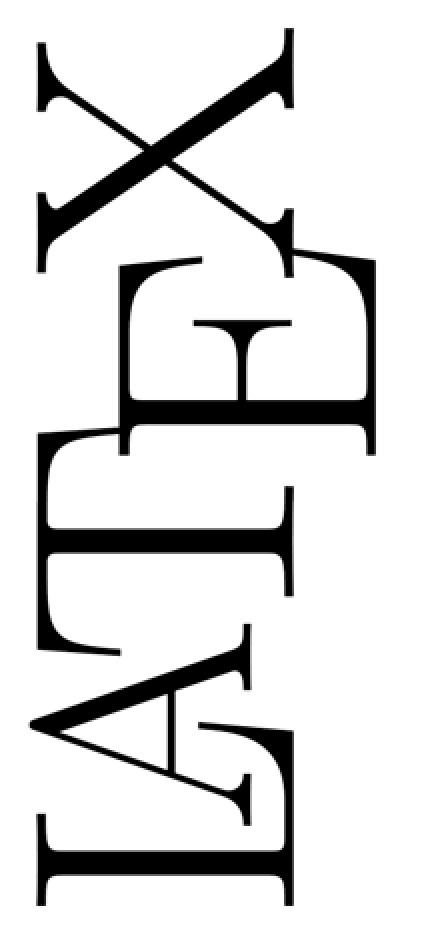
\includegraphics[scale=0.27]{latex}
  }
  \caption{Первая нейросетевая языковая модель}\label{fig:Neuro1-Feedforward}
\end{figure}


\section{Векторные представления слов}
Разреженные представления слов в обработке естественного текста использовались достаточно давно. Хотя, как было показано выше, плотные представления слов для языкового моделирования предлагались еще в 2001 году, основное нововведение \cite{Mikolov_Chen_Corrado_Dean_2013}, предложенное в 2013 году Миколовым, - архитектура word2vec - позволило гораздо успешнее обучать векторные представления слов. Word2vec существует в двух вариантах - CBOW и skip-gram, которые подробнее представлены на рисунке 6. Они различаются по своей цели: один предсказывает центральное слово на основе окружающих слов, а другой делает обратное.


\begin{figure}[ht]
  \centerfloat{
    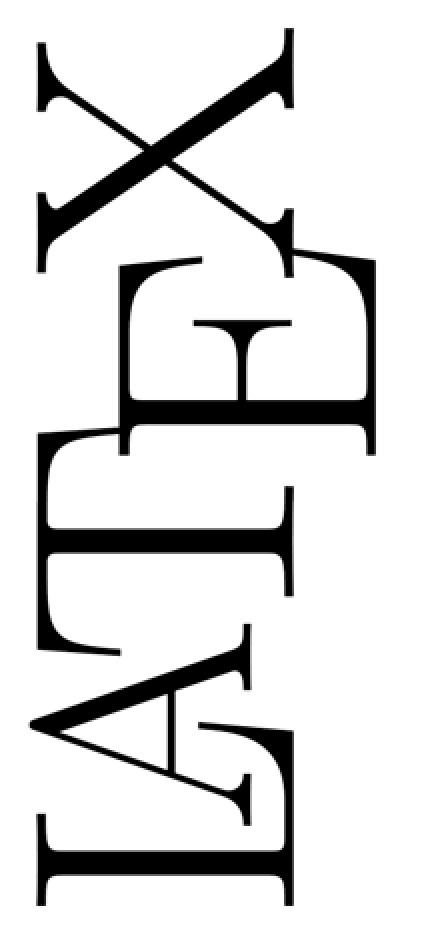
\includegraphics[scale=0.27]{latex}
  }
  \caption{Word2Vec}\label{fig:Neuro2-Word2Vec}
\end{figure}

Обучение модели на большом корпусе позволяет модели выучить такие понятия, как пол, время глагола, или отношения типа страна-столица. Различные, более сложные методы векторизации слов (fasttext, glove, elmo и пр.), широко применяются и по сей день, так как их использование улучшает качество решения многих задач машинного обучения.


\section{Нейронные сети для обработки текста}
В 2013-2014 годах нейросети (в первую очередь - рекуррентные, сверточные и рекурсивные) стали активно использоваться для обработки текста.  Наиболее широко в то время использовались три основных типа нейронных сетей: рекуррентные нейронные сети, сверточные нейронные сети и рекурсивные нейронные сети. Они будут подробнее описаны ниже.

\section{Рекуррентные нейронные сети}
Рекуррентные нейронные сети (RNN) лучше всего подходят для работы с динамическими входными последовательностями, из которых и состоит естественный язык.  Первые рекурсивные сети были предложены Элманом в 1990 году \cite{Elman_1990}, но в 1997 году на их место пришли предложенные Шмитхубером сети долговременной памяти(LSTM) \cite{Hochreiter_Schmidhuber_1997}, которые оказались более устойчивыми к проблеме исчезания/взрыва градиентов. В 2013 году Илья Суцкевер предложил в своей диссертации новый, более эффективный метод обучения LSTM \cite{Suskever_2013}. Также в 2013 году Грэйвсом были предложены двунаправленные LSTM \cite{Graves_Jaitly_Mohamed_2013}, которые обычно используется для работы с левым и правым контекстом. Визуализацию ячейки LSTM можно увидеть на рисунке 7.  


\begin{figure}[ht]
  \centerfloat{
    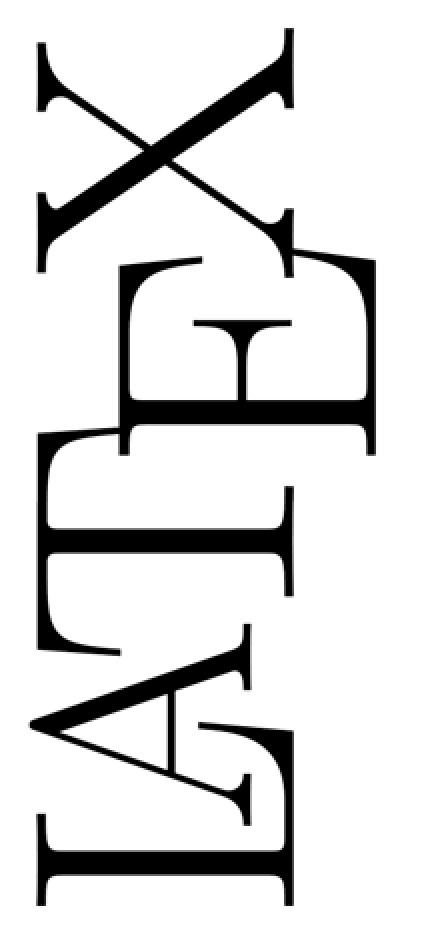
\includegraphics[scale=0.27]{latex}
  }
  \caption{Визуализация ячейки LSTM}\label{fig:Neuro3-LSTM}
\end{figure}


\section{Сверточные нейронные сети}
Сверточные нейронные сети работают на основе операции свертки в двух измерениях, в 2014 году \cite{Kalchbrenner_Grefenstette_Blunsom_2014} они начали применяться в области обработки естественного языка. Преимуществом сверточных нейронных сетей, по сравнению с рекуррентными, является их распараллеливаемость. На рисунке 8 показан пример сверточной нейронной сети, используемой в обработке текста.


\begin{figure}[ht]
  \centerfloat{
    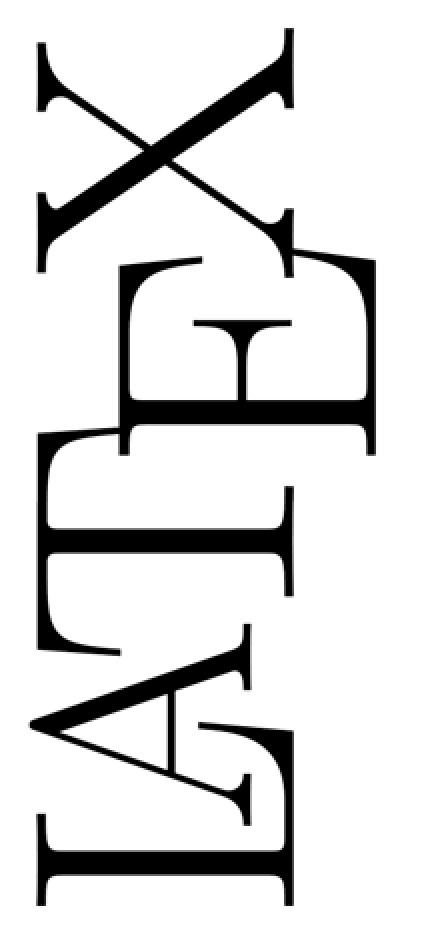
\includegraphics[scale=0.27]{latex}
  }
  \caption{Пример сверточной нейронной сети}\label{fig:Neuro4-CNN}
\end{figure}

\section{Рекурсивные нейронные сети}
Хотя рекуррентные и сверточные нейросети рассматривают естественный язык как последовательность, по своей сути он иерархичен: слова состоят из фраз и предложений более высокого порядка, которые сами могут быть рекурсивно объединены в соответствии с набором строго определенных правил. Это приводит к идее трактовать предложения как деревья, а не как последовательности. Воплощением данной идеи являются рекурсивные нейронные сети \cite{Socher_Perelygin_Wu_Chuang_Manning_Ng_Potts_2013}. В отличие от рекуррентных сетей, обрабатывающих предложение слева направо или справа налево, рекурсивные сети представляют последовательность снизу вверх или сверху вниз. Новое представление в каждом узле находится при помощи составления представлений дочерних узлов. Пример рекурсивной нейронной сети изображен на рисунке 9.



\begin{figure}[ht]
  \centerfloat{
    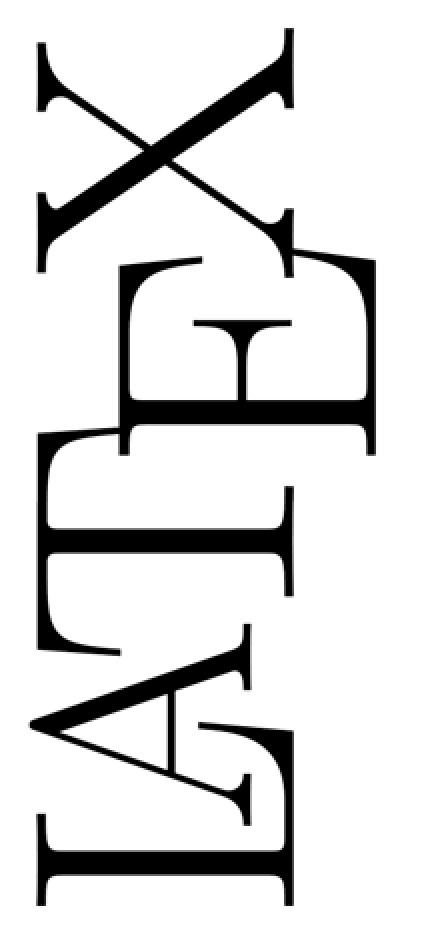
\includegraphics[scale=0.27]{latex}
  }
  \caption{Пример рекурсивной нейронной сети}\label{fig:Neuro5-RNN}
\end{figure}

\section{Seq2Seq  модели}
     В 2014 году Илья Суцкевер предложил методику обучения Seq2Seq моделей \cite{Sutskever_Vinyals_Le_2014} - нейросетевых моделей для отображения одной последовательности в другую. В данных моделях нейросеть энкодера обрабатывает каждый токен предложения по очереди  и сжимает их в вектора скрытых состояний; на основе этих векторов скрытых состояний нейросеть декодера шаг за шагом прогнозирует символ энкодера, который предполагается на выходе. Пример работы данной сети изображен на рисунке ~ref.

\begin{figure}[ht]
  \centerfloat{
    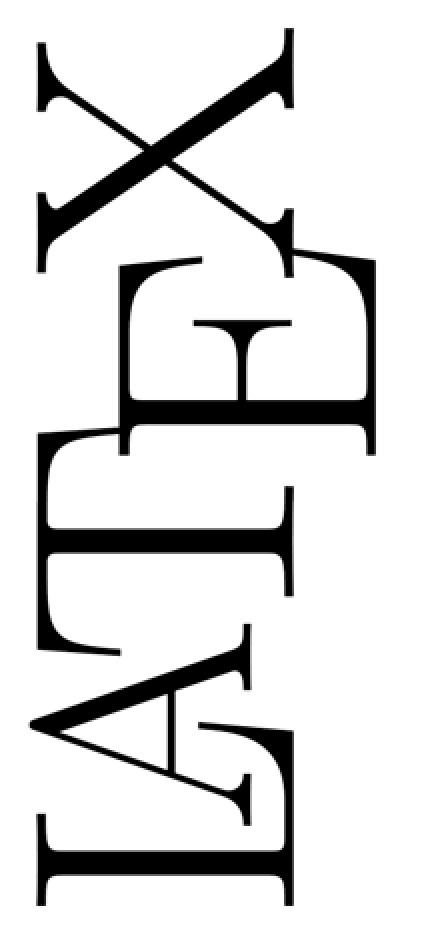
\includegraphics[scale=0.27]{latex}
  }
  \caption{Пример сети на основе модели Seq2Seq}\label{fig:Neuro6-Seq2Seq}
\end{figure}


    В 2016 году Google начал заменять свои модели машинного перевода на Seq2Seq модели. По словам Джеффа Дина, это означало замену 500 000 строк кода, сопоставляющего паттерны,  моделью нейронной сети на 500 строк. Seq2Seq модели могут широко применяться в любых задачах, где данные имеют конкретную структуру.
    
Обычно архитектура энкодера и декодера основана на рекуррентных нейронных сетях, но периодически появляются новые архитектуры. Обычно они обкатываются на задаче машинного перевода. Энкодер и декодер могут быть основаны на нейросетях с долгосрочной памятью, сверточных сетях, трансформерах(которые будут подробно описанных в следующей главе) и пр.

\section{Нейросети, основанные на памяти}
В середине 2010-х годов стали активно появляться архитектуры нейросетевых моделей, использующие память - скрытые состояния модели, при этом модель сама выбирает, что необходимо извлечь из памяти. 
     Внимание можно рассматривать как форму нечеткой памяти, где память состоит из прошлых скрытых состояний модели, причем модель выбирает, что извлечь из памяти.  Из моделей, использующих память, можно выделить сквозные сети памяти \cite{Sukhbaatar_Szlam_Weston_Fergus_2015}, модели с динамической памятью \cite{Kumar_Irsoy_Ondruska_Iyyer_Bradbury_Gulrajani_Zhong_Paulus_Socher_2016}, дифференцируемые нейрокомпьютеры \cite{Graves_Wayne_Reynolds_Harley_Danihelka_Grabska-Barwińska_Colmenarejo_Grefenstette_Ramalho_Agapiou_et al._2016}, модели с памятью "ключ-значение" \cite{Miller_Fisch_Dodge_Karimi_Bordes_Weston_2016} и пр.
 
     Доступ к памяти в таких моделях осуществляется при помощи "похожести" по текущему расстоянию по той или иной метрике, подобным вниманию, и память в модели обычно может записываться и считываться.  Модели отличаются тем, как они реализуют и используют память. Например, сквозные сети памяти обрабатывают ввод несколько раз и только затем обновляют память, чтобы сделать возможным несколько этапов вывода.  Нейронные машины Тьюринга имеют адресацию на основе местоположения, что позволяет им изучать простые компьютерные программы, такие как сортировка.  Модели на основе памяти, как правило, применяются к задачам, где информацию нужно хранить достаточно долго, например, моделирование языка или понимание текста.  
